\chapter{Construcción y Caracterización de los Biosensores}
\label{cap:Biosensores}

Teniendo en cuenta un esquema simplificado de la red apoptótica, podemos apreciar que como mínimo nos interesaría poder visualizar la actividad de tres nodos, uno en cada módulo. Dado que cada uno se caracteriza por tener al menos una caspasa, podemos utilizar tres sensores análogos que sean sensibles a distintas proteasas. Además, para poder ubicar los tres sensores en el espectro accesible por las cámaras del microscopio, necesitaremos que los fluoróforos estén basados en homoFRET. Si considerásemos sensores basados en heteroFRET, cada sensor necesita un rango del espectro para el dador y el aceptor separados, imposibilitando el uso de más de dos biosensores simultáneamente. En este capítulo detallaré cómo se seleccionaron los pares de fluoróforos para construir los biosensores \citep{Corbat2018}. Finalmente, dado que los biosensores añadidos de forma exógena en las células introducen perturbaciones en la red estudiada, se caracterizó y redujo la variabilidad introducida en el sistema \citep{Habif2021}.

\section{Selección de Especies de Fluoróforos}

A partir de datos preliminares del grupo, se utilizaron tres pares de fluoróforos cuyos espectros prácticamente no se superponen entre si. Dicho estudio comenzó con un análisis de la distancia de Förster ($R_0$) característica de distintos pares de fluoróforos. Se generaron los constructos en tandem de las combinaciones con mayor $R_0$ y se evaluó experimentalmente la anisotropía del dímero y monómero. Cabe destacar que en los extremos del espectro, rango de los azules y rojos, es difícil encontrar un par de fluoróforos idénticos con elevado rango dinámico de valores de anisotropía. Por esta razón, se consideraron fluoróforos distintos con espectro de excitación y emisión similares. Esto trae aparejada la ventaja que los valores de anisotropía están dados, no solo por los cambios de polarización, sino también por los cambios en la detección. Es decir, la anisotropía dependerá también de la combinación de filtros y lentes utilizados (ver \cref{fig:fluopairs}).

\begin{figure}[t!]
    \centering
    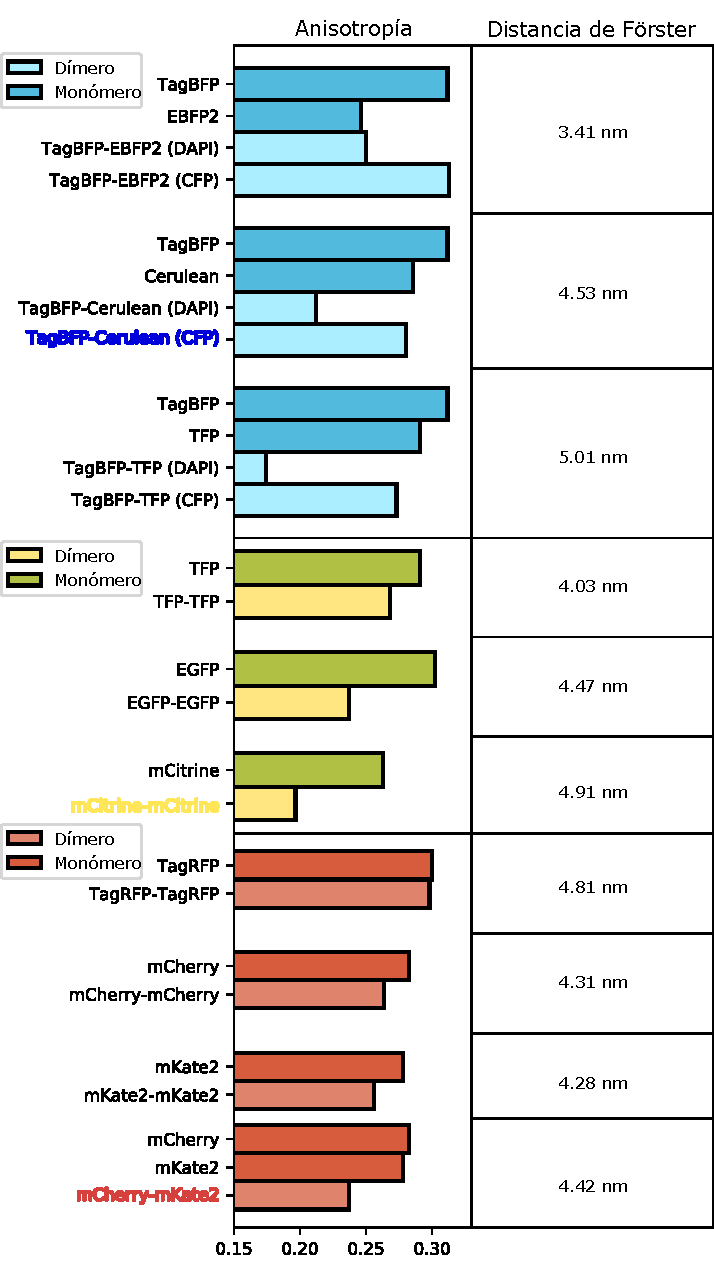
\includegraphics[width=0.6\textwidth]{img/cap_3/fluorophore_pairs.pdf}
    \caption{\footnotesize{Se muestran las anisotropías medidas experimentalmente de los distintos pares de fluoróforos evaluados, así como las distancias de Förster calculadas para cada par. Se debe destacar que cuando fue posible, se midió la anisotropía utilizando un conjunto de filtros distintos ya que éstos afectarán la anisotropía detectada. Notar que en los extremos del rango visible se utilizaron fluoróforos distintos ya que las diferencias en detección mejoraban la anisotropía observada. Adaptado de \cite{Corbat2018}.}}
    \label{fig:fluopairs}
\end{figure}

Varias de las combinaciones de fluoróforos generados exhibieron un elevado cambio en anisotropía. Hubieron otras combinaciones cuyo cambio no fue tan notorio, probablemente por efecto de una orientación desfavorable entre los fluoróforos que no podría haber sido tenido en cuenta en los cálculos. Es así que las tres combinaciones seleccionadas fueron: TagBFP-x-Cerulean, mCitrine-x-mCitrine y mCherry-x-mKate2, donde la x puede ser reemplazada por cualquier secuencia sensible a ser clivada. Los filtros utilizados para la adquisición fueron: 377/28 y 460-510 para excitación y emisión del canal azul, 495/10 y 515-560 para el verde y 545-580 y un long pass de 610 para el canal rojo (ver \cref{fig:fluospectra}). Notar que dadas las superposiciones entre filtros, no es posible adquirir simultáneamente todos los canales, pero sí secuencialmente sin que haya un sangrado apreciable entre los canales.

\begin{figure}[t!]
    \centering
    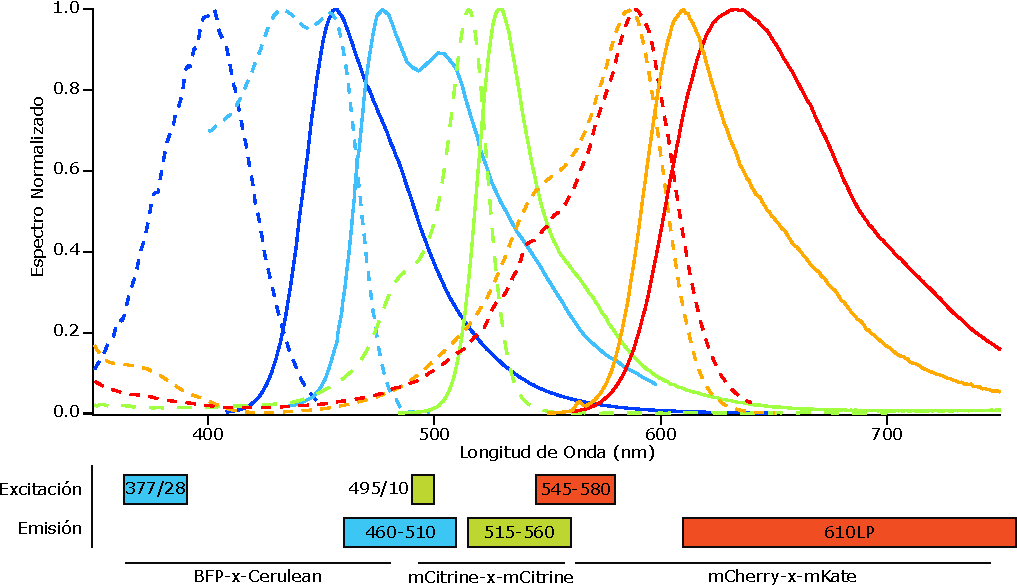
\includegraphics[width=0.9\textwidth]{img/cap_3/fluospectra.pdf}
    \caption{\footnotesize{Espectros de excitación y emisión de los fluoróforos seleccionados. En la sección inferior se muestran los filtros de ecitación y emisión utilizados para cada par de fluoróforos. Si se hace una adquisición secuencial no es necesario corregir sangrado espectral entre canales. Adaptado de \cite{Corbat2018}.}}
    \label{fig:fluospectra}
\end{figure}

Habiendo identificado los pares de fluoróforos con mayor rango dinámico en anisotropía de polarización, resta elegir la secuencia de unión entre ambos, en nuestro caso, la caspasa a la que será sensible. Debido a la facilidad con que se pueden intercambiar los pares y secuencias, se utilizaron varias combinaciones a lo largo de la tesis.

Desde un punto de vista evolutivo, la cascada apoptótica está bastante conservada. A lo largo de la evolución de caspasas, estas aumentaron en cantidad y funcionalidad dependiendo del organismo en cuestión. Aunque cada caspasa tiene especificidad por ciertas secuencias de aminoácidos, algunas caspasas comparten ésta especificidad. Por ejemplo, las caspasas efectoras 3 y 7 clivan en el dominio DEVD. Por otro lado, las caspasas iniciadoras 8 y 9 reconocen los sitios IETD y LEHD, respectivamente \citep{Sakamaki2009}. Sabiendo esto, las variantes se denominarán acorde a la caspasa siendo sensada y el color del par de fluoróforos utilizado. Siguiendo la denominación de las publicaciones sCasx-FP, donde x corresponde a la caspasa sensada: caspasa 3 para DEVD, caspasa 8 para IETD-IETD y caspasa 9 para LEHD; mientras que FP (por las siglas de \ening{fluorescent pair}) será reemplazado por RP, GP o BP según sea el par rojo, verde o azul, respectivamente (por sus siglas en inglés).

Los biosensores se construyeron insertando el segundo fluoróforo amplificado por PCR y delimitado por los sitios de restricción de Spe1 y Sal1 y conteniendo un codón STOP en los sitios de restricción Spe1/Sal1 de un vector-C1 (Clontech). Adicionalmente, el producto de PCR tenía una secuencia de unión en el extremo 5'. Estos plásmidos se utilizaron como controles no clivables. Por otro lado, para construir los sensores clivables por la caspasa, se utilizaron las secuencias que codificaban para los sitios de clivado de las caspasas amplificadas por PCR y delimitadas por sitios de restricción BSP1 y Spe1, y luego subclonados a los sitios de restricción correspondientes en los plásmidos de control no clivables, volviéndolos plásmidos que codifican para el sensor clivable.


%%%%%%%%%%%%%%%%%%%%%%%%%%%%
\section{Estimación de la Anisotropía del Dímero y del Monómero}


Para poder estimar la actividad de la caspasa a partir de las curvas de anisotropía es necesario estimar los valores de anisotropía del monómero y dímero de cada par de fluoróforos. Para ello, se tomaron las curvas medidas experimentalmente y se seleccionó mediante máscaras la región correspondiente al momento en que transcurre la apoptosis. Se tomó un promedio de los cinco valores de anisotropía previos al inicio de la máscara y posteriores para estimar la anisotropía del dímero y monómero, respectivamente. Dado que los valores estimados para cada curva tenían mucha variabilidad, y considerando las fuentes de error en su estimación (ver sección \ref{sec:matmet:CalculoAnisotropia}), se decidió estimar dichos valores para cada curva en lugar de utilizar un único valor para cada par de biosensores. De todas formas, se corroboró que en todos los casos la diferencia de anisotropía era positiva y de un valor distinguible del ruido experimental (ver \cref{fig:anisotropy_histogram}).

\begin{figure}
    \centering
    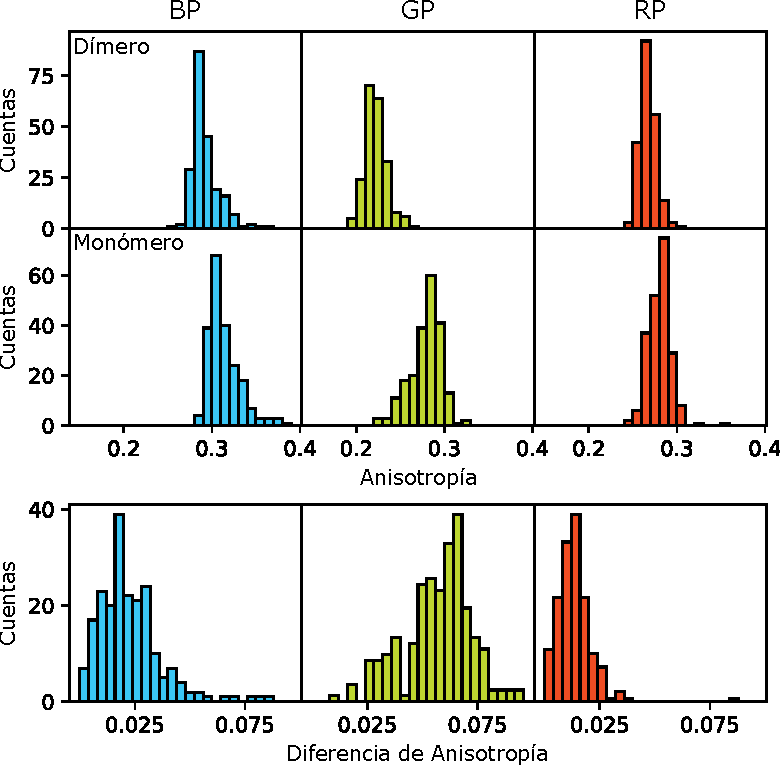
\includegraphics[width=0.7\textwidth]{img/cap_3/anisotropy_histograms_all.pdf}
    \caption{\footnotesize{Histogramas correspondientes a las anisotropías del monómoero y dímero estimadas a partir de 212 curvas. Para cada biosensor, los histogramas de la anisotropía del dímero y monómero se superponen bastante, mientras que en los histogramas de las diferencias se ve que todos los valores son positivos. Adaptado de \cite{Habif2021}.}}
    \label{fig:anisotropy_histogram}
\end{figure}


%%%%%%%%%%%%%%%%%%%%%%%%%%%%
\section{Calibración del Parámetro \texorpdfstring{$\Delta b$}{Deltab}}


Habiendo seleccionado los pares de fluoróforos a utilizarse, debemos hallar el valor de $\Delta b$ correspondiente a cada par. La calibración más directa que a uno se le puede ocurrir es obtener los valores de brillo por cada tipo de molécula para determinar así los valores de $b$ y $\Delta b$. Sin embargo, esto no siempre es posible ni la mejor forma. Otra posibilidad consiste en generar biosensores con los tres pares de fluoróforos pero que sensen la misma caspasa. Como la caspasa no tiene ninguna preferencia por ninguno de los tres sensores, las curvas de los tres deberían corresponder a curvas de actividad idénticas, así como la diferencia entre los máximos de actividad debería ser nula.

\begin{figure}
    \centering
    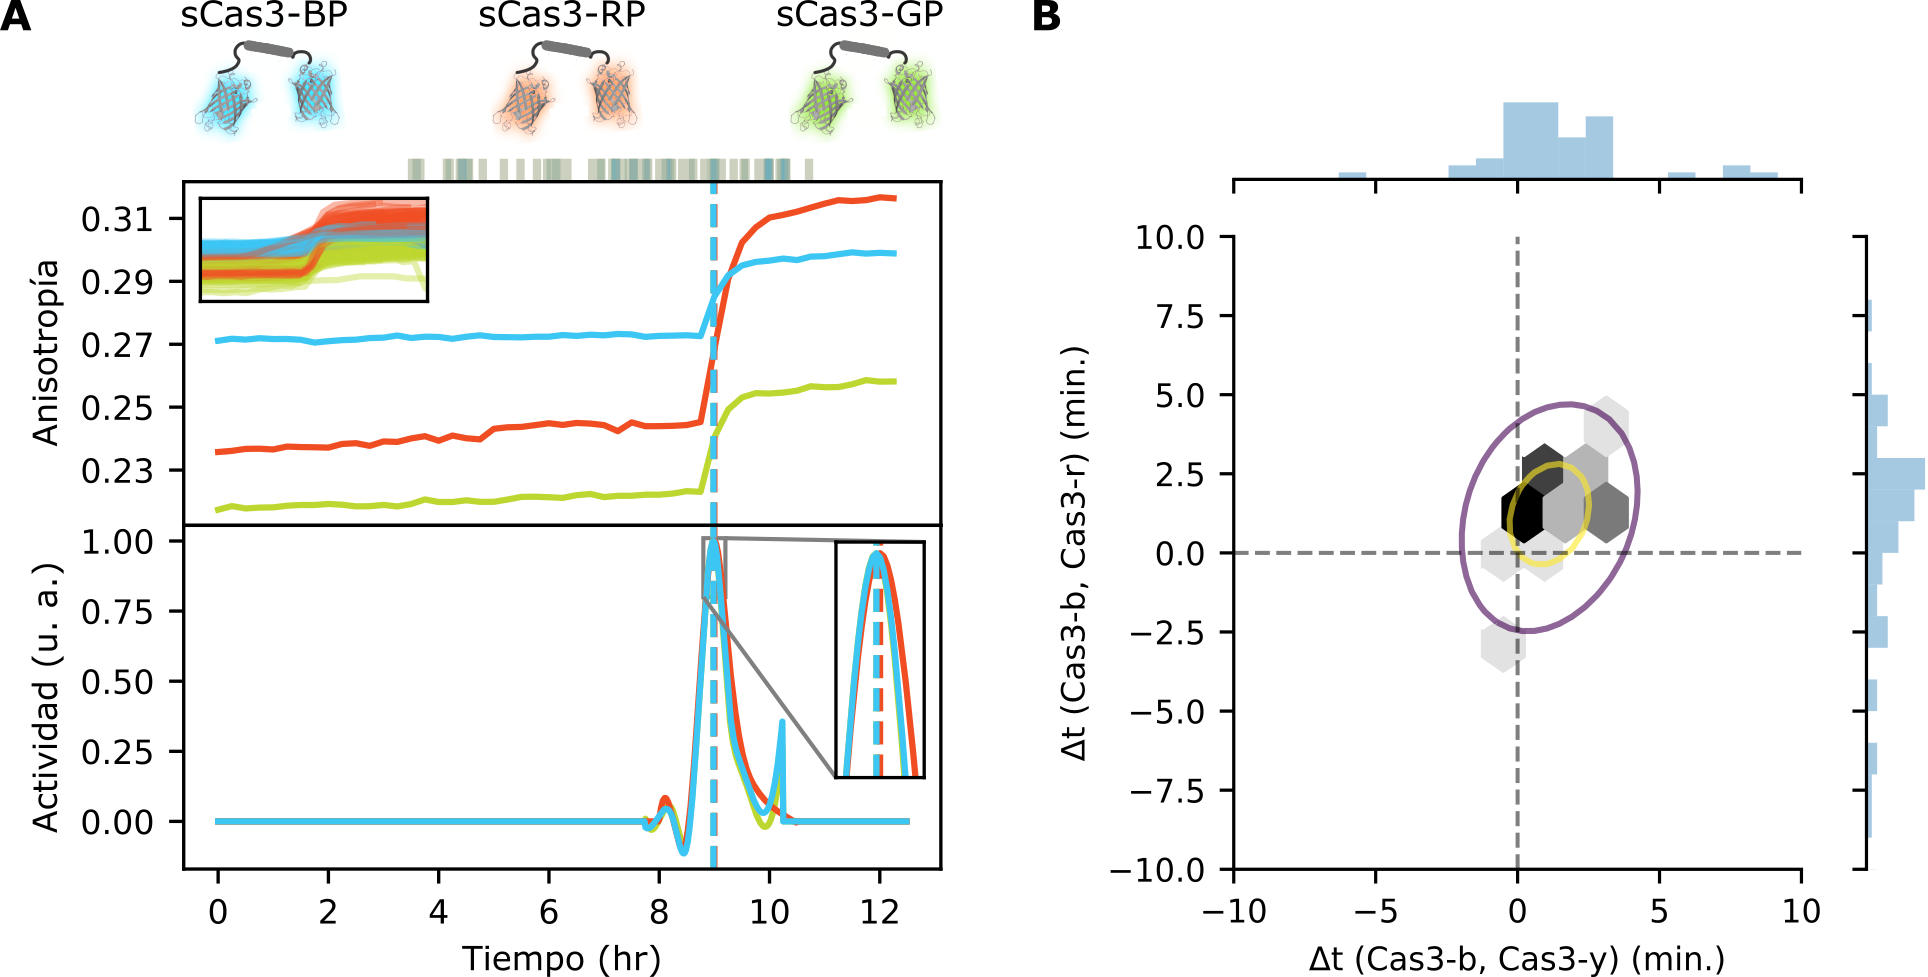
\includegraphics[width=0.9\textwidth]{img/cap_3/onecasp.png}
    \caption{\footnotesize{Se transfectaron a células HeLa los biosensores sCas3-RP, sCas3-GP y sCas3-BP y se las estimuló con staurosporina (N=54). Adaptado de \cite{Corbat2018}. \textbf{A.} Se muestra a modo de ejemplo tres curvas de anisotropía con sus correspondientes curvas de actividad. En la sección superior cada varilla representa el instante de máxima actividad observado para alguna de las 54 células analizadas. Todas las curvas de anisotropía se graficaron superpuestas en el recuadro superior, mientras que el recuadro inferior contiene una sección amplificada de la región de los máximos. \textbf{B.} Histograma bidimensional en donde se muestran las diferencias de tiempo entre los biosensores en forma de hexágonos. Las curvas de nivel se obtienen de un gráfico de estimación de densidad de kernel y encierran el 34\% (amarillo) y 68\% (violeta) de los datos. El gráfico superior y derecho son las distribuciones marginales de las diferencias de tiempo.}}
    \label{fig:onecasp}
\end{figure}

Para calibrar los pares de fluoróforos utilizados, se transfectaron a las células los sensores sCas3-RP, sCas3-GP y sCas3-BP. Para inducir apoptosis, se utilizó una concentración 1~$\mu$M de staurosporina. Siguiendo el protocolo experimental delineado en el \cref{cap:MatMet}, se obtuvieron y analizaron las sucesivas imágenes tomadas en un lapso de 15~hr. A partir de las curvas de anisotropía generadas, se estimaron las correspondientes curvas de actividad de la caspasa y se recuperó para cada una el tiempo de máxima de actividad (ver \cref{fig:onecasp}A). A continuación, se buscaron los valores de $\Delta b$ que minimicen las diferencias entre tiempos de máxima actividad, obteniéndose 0.15 para BP, 0.17 para GP y -0.15 para RP. Se presenta un histograma bidimensional en la \cref{fig:onecasp}B de los valores de los tiempos obtenidos.


%%%%%%%%%%%%%%%%%%%%%%%%%%%%
\section{Perturbación de los Biosensores}


Hasta ahora hemos modelado e imaginado a los biosensores y sus caspasas separadas en un modelo simple, pero en realidad, éstas son parte de una cascada de señalización dentro de la célula y los sensores son añadidos de forma exógena. Como cualquier especie agregada, ésta competirá por la enzima con las especies endógenas y propias del sistema. Esto quiere decir que la propagación de la señal a través de la red puede verse demorada por un efecto de secuestro de las caspasas por parte de los biosensores. Este efecto se torna más importante ya que depende de la concentración y los biosensores transfectados se hallan en concentraciones elevadas debido a que el promotor viral (CAG) hace que sean sintetizados constantemente \citep{Wachsmuth2015}. 

Al transfectar cada biosensor en un plásmido distinto, cada uno tiene cierta probabilidad de ser efectivamente incorporado a la célula \citep{Schwake2010}. Esto se traduce en que habrán células transfectadas con uno o dos de las variantes de biosensores en lugar de los tres, así como células que tendrán uno en exceso y los otros biosensores en menor concentración. Este fenómeno combinado con el efecto de secuestro de cada biosensor se traduce en que la demora introducida en cada nodo sensado de la red será distinta de célula a célula, dependiendo de como fue la transfección.

Surgieron varias estrategias para mejorar la co-expresión de proteínas: desde utilizar múltiples promotores \citep{Kriz2010}, promotores bidireccionales \citep{Vogl2018}, sitios internos de entrada al ribosoma (IRES por sus siglas en ingles, \cite{Wong2002}) o el uso de secuencias virales de péptidos 2A \citep{Kim2011}. Aunque utilizar múltiples promotores asegura una expresión elevada de los genes transfectados, no asegura la estequiometría en la expresión. Los promotores bidireccionales traen aparejada la dificultad de su construcción así como su cantidad limitada de genes. Por otro lado, las secuencias de IRES suelen tener más de 800 pares de bases y es sabido que secuencias muy extensas traen aparejados otros problemas al momento de expresarse. Por último, las secuencias virales 2A emergieron en la última década y consisten en secuencias \textit{auto-clivables} de alrededor de 20 aminoácidos. 

El mecanismo por el cual las secuencias 2A se clivan es un evento de hidrólisis co-transduccional entre los residuos de glicina y prolina de una secuencia conservada (Asp-Val/Ile-Glu-X-Asn-Pro-Gly-¯-Pro), dando lugar a la expresión de proteínas distintas a partir de un único ARN mensajero. Específicamente, se impide la formación de una unión peptídica normal vía un ``salto ribosomal'' sin afectar la traducción de la proteína codificada río abajo \citep{Szymczak2005}. En el trabajo de \cite{Szymczak2004}, se utiliza un plásmido multicistrónico codificando para las cuatro subunidades del complejo CD3 y así restaurar el desarrollo de células T en ratones deficientes de dicho complejo. Además de ser útiles para expresar subunidades de complejos, pueden ser implementadas para expresar diversos reporteros como muestran \cite{Levin2014} al utilizarlas para expresar una proteína fluorescente, una luciferasa para detección mediante bioluminiscencia y una quinasa de timidina para poder visualizarla a través de tomografía de emisión de positrones.

Luego de haber identificado el impacto de la concentración de los biosensores, se comenzó el diseño de una estrategia para controlar la estequiometría de los biosensores. La caracterización de dicha implementación fue realizada en conjunto con el Dr. Martín Habif en el Laboratorio de Electrónica Cuántica; y en viajes que realizamos al Instituto Pasteur de Montevideo (Uruguay) y Max Planck Institute for Molecular Physiology (Dortmund, Alemania). A continuación, se trabajo en conjunto para estudiar el efecto de dicha modificación en la variabilidad de los observables biológico y analizar los datos de todos los experimentos realizados.


%%%%%%%%%%%%%%%%%%%%%%%%%%%%
\section{Construcción de CASPAM}


Con el objetivo de reducir la variabilidad en la estequiometría de los sensores y basándonos en el trabajo de \cite{Goedhart2011}, donde se muestra que utilizar secuencias virales 2A resulta en una mayor correlación en la concentración de dos fluoróforos, se implementó un plásmido multicistrónico donde cada biosensor se halla separado por dichas secuencias. Para su confección, se tomaron los tres sensores de actividad caspasa (CAS, por sus siglas en inglés) y se los arregló en tandem utilizando secuencias flexibles (GGGSGGG) y virales 2A (P2A: \seqsplit{ATNFSLLKQAGDVEENPGP} y T2A: \seqsplit{EGRGSLLTCGDVEENPGP}) entre ellos. La elección de las secuencias estuvo guiada por el trabajo de \cite{Liu2017} donde muestran como la eficiencia de auto-clivaje decrece en el orden P2A\textless T2A\textless E2A\textless F2A. Se reemplazaron todos los codones STOP con glicina a excepción del fluoróforo ubicado en el extremo 3' del constructo. Finalmente, el gen sintético de $\sim$5kb fue clonado entre los sitios de restricción KpnI/EcoRI de un vector pcDNA3.1(+) (Life Technologies, Grand Island, NY). La combinación de sensores seleccionados fue sCas3-GP, sCas8-BP y sCas9-RP y el control de la traducción está regido por un promotor de Citomegalovirus (CMV). La integridad de cada cassette en mCitrine-DEVD-mCitrine-P2A-tagBFP-IETD-Cerulean-T2A-mCherry-LEHD-mKate fue confirmada por secuenciación en el constructo final. Considerando que los tres biosensores pueden ser multiplexados mediante anisotropía de polarización, se nombró al constructo CASPAM, por sus siglas en inglés \textit{Caspase Activity Sensor by Polarization Anisotropy Multiplexing} (ver \cref{fig:secuencia}).

\begin{figure}[htb]
    \centering
    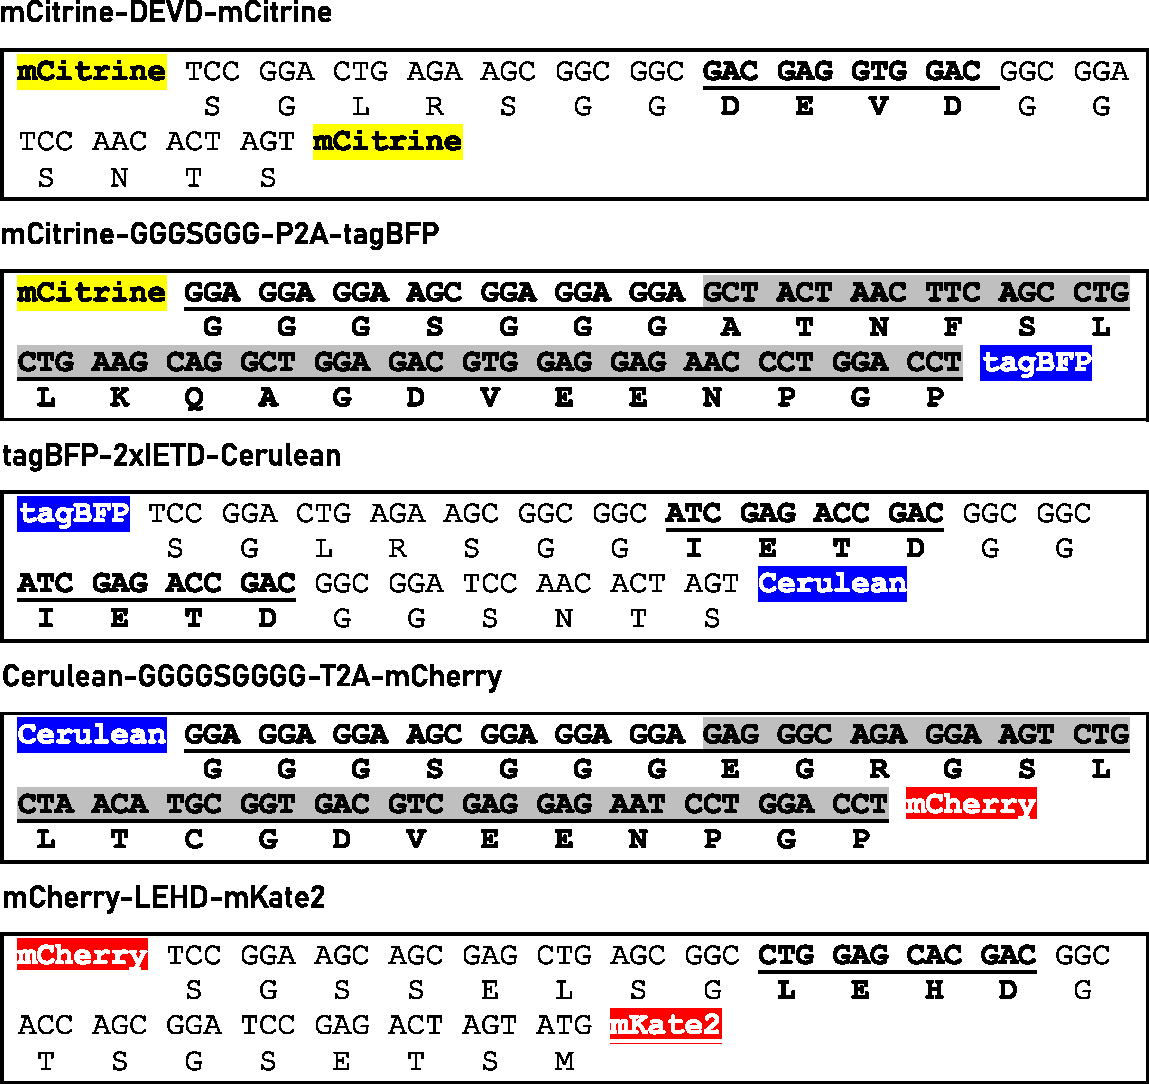
\includegraphics[width=0.7\textwidth]{img/cap_3/CASPAM_seq.pdf}
    \caption{\footnotesize{Secuencia de CASPAM. Se pueden apreciar los tres biosensores sCas3-GP, sCas8-BP y sCas9-RP separados por secuencias virales 2A y secuencias flexibles compuestas por GGGSGGG. Adaptado de \cite{Habif2021}.}}
    \label{fig:secuencia}
\end{figure}

Luego, se verificó la expresión de los biosensores a partir de la transfección de CASPAM en células HeLa. Una vez transfectadas, se las incubó por 24~hr y se las sometió a Western Blot. Este procedimiento permite inferir a partir de la distancia recorrida desde su punto de siembra el peso molecular de la proteína de interés. El no haber detectado bandas en las regiones de peso molecular equivalente al de tres biosensores ($\sim$170~kD) ni dos biosensores ($\sim$110~kD) confirma que no se hallan subproductos correspondientes a un clivaje incompleto entre biosensores (ver \cref{fig:transfeccion}A). Contrario a esto, se pudo apreciar una banda intensa correspondiente al peso molecular de un dímero de fluoróforos ($\sim$52~kD), que además confirma que no se hallan biosensores clivados por caspasas en condiciones sin perturbar.

\begin{figure}
    \centering
    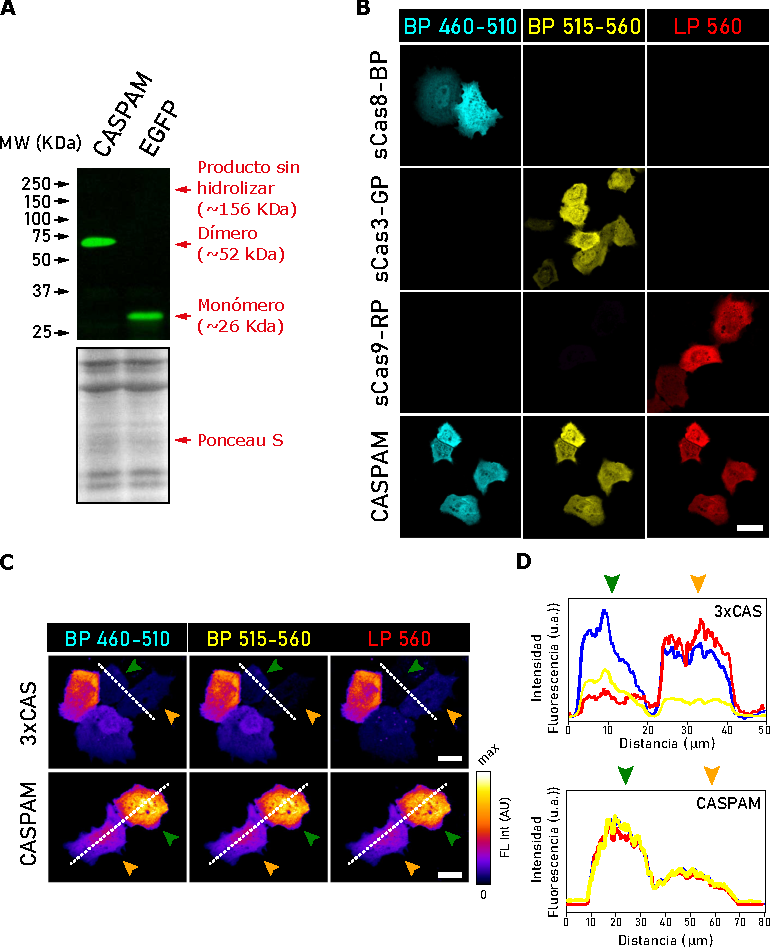
\includegraphics[width=0.8\textwidth]{img/cap_3/transfeccion.pdf}
    \caption{\footnotesize{Se transfectaron células HeLa con CASPAM y se corroboró la síntesis de los biosensores. Adaptado de \cite{Habif2021}. \textbf{A.} Se realizó un Western Blot y se lo marcó con anticuerpos anti-GFP. Éstos anticuerpos se pueden visualizar mediante fluorescencia y se unen tanto a GFP como a mCitrine y CFP. Se puede apreciar que en el carril de células transfectadas con EGFP se ve una única marca correspondiente a un único fluoróforo, mientras que en las células transfectadas solo se ve una marca en el doble de peso molecular. Al no verse marcas en tamaños mayores, interpretamos que no hay productos sin hidrolizar. En la imagen inferior se ve una tinción con Ponceau S que sirve para estimar pesos moleculares sin afectar las proteínas del gel. \textbf{B.} Células transfectadas con los tres sensores por separado o con CASPAM y luego fijadas fueron analizadas por microscopía confocal. Se puede apreciar que no hay sangrado espectral entre los distintos canales, así como que las células transfectadas con CASPAM expresan lo tres biosensores. \textbf{C.} Imágenes de microscopía confocal de las células transfectadas con 3xCAS y CASPAM. Los perfiles de intensidad de las rectas se muestran en \textbf{D}. Aunque las intensidades de los biosensores transfectados con CASPAM varían de célula a célula, éstos no varían tanto entre canales de la misma célula. En contraposición, las células transfectadas con 3xCAS presentan una elevada variabilidad en la intensidad intercanal e intercelular.}}
    \label{fig:transfeccion}
\end{figure}

Más allá de de la presencia de los biosensores dentro de las células, se corroboró por medio de microscopía de fluorescencia que los tres biosensores se encuentren en células únicas y que su plegado sea el correcto, dando lugar a emisión de fluorescencia. Para ello se transfectaron células HeLa con una mezcla de plásmidos codificando para 3 CAS (sCas3-GP, sCas9-BP, sCas8-RP) o con CASPAM y se las fijó con paraformaldehído 24~hr después. Se utilizó microscopía confocal para observar la emisión de los fluoróforos en los distintos canales, y como se esperaba, no se detectó ningún sangrado entre ellos (ver \cref{fig:transfeccion}B). Adicionalmente, las células transfectadas con CASPAM no sólo mostraban fluorescencia en los debidos canales, sino que también mostraban muy poca variabilidad en intensidad intercanal aunque sí variabilidad intercelular. Esto sugiere que la estequiometría entre los biosensores esta mejor conservada al utilizar CASPAM (ver \cref{fig:transfeccion}C y D).


%%%%%%%%%%%%%%%%%%%%%%%%%%%%
\section{Caracterización de la Expresión de CASPAM}


A continuación, se utilizó citometría de flujo para caracterizar los niveles de fluorescencia de una gran población de células (FACS) y espectroscopia de correlación de fluorescencia (FCS) para poder determinar adecuadamente la estequiometría. FACS consiste en hacer pasar del orden del miles de células de a una por un sistema óptico que permite clasificar y caracterizar cada una según sus propiedades ópticas y de fluorescencia. En cuanto a FCS, es una técnica basada en microscopía confocal de detección de molécula única donde se analizan las correlaciones en fluctuaciones de intensidad generadas por partículas fluorescentes entrando y saliendo de un volumen de observación del orden de un femtolitro \citep{Digman2008}. Cabe destacar que FACS es una técnica extensiva en cuanto a que describirá miles de células, mientras que FCS requiere varias repeticiones de la medición de cada punto por lo que no es posible describir tantas células. Otra diferencia importante es el rango dinámico de cada una, ya que FACS puede reportar niveles de fluorescencia con varios ordenes de magnitud de diferencia, mientras que FCS depende de los parámetros microscopio utilizado y es mucho menor. Para ambos experimentos, se transfectaron nuevamente células HeLa con 3xCAS y CASPAM y se analizaron 24~hr post transfección. Además, FACS refiere a la fluorescencia detectada en cada célula y por lo tanto su relación no nos brinda información sobre cual es la estequiometría, sino cuanto varía ésta entre células. A partir de FCS podemos estimar la cantidad de moléculas dentro del volumen confocal y así calcular la estequiometría entre los sensores.


\subsection{Clasificación de Células por Fluorescencia Activada}


Además de las células transfectadas con 3xCAS y CASPAM, se analizaron células transfectadas con: i) sCas3-GP, ii) sCas8-RP, iii) sCas9-BP, iv) sCas3-GP + sCas8-RP, v) sCas3-GP + sCas9-BP, vi) sCas8-RP + sCas9-BP. Se utilizó un citómetro FACS-Aria Fusion (BD Biosciences) equipado con láseres de 405~nm, 488~nm y 561~nm. Se cuantificó la emisión de fluorescencia utilizando los filtros BP450/50 (verde), BP530/30 (azul) y BP610/20 (rojo). Para cada muestra se dejó pasar un total de $2 \times 10^4$ cuentas en gráfico de puntos de forward scatter (FSC) versus side scatter (SSC), excluyendo dobletes. Los datos se adquirieron por medio de CellQuest software (BD Biosciences) y se procesaron con FlowJo v7.6.5 software.

Los análisis de FACS de células transfectadas con un vector vacío y con un único plásmido que codifique para un único biosensor sirvieron de calibración (ver \cref{fig:FACS_singles}). Los niveles de fluorescencia detectados en las células que fueron transfectadas con el vector vacío se corresponden con autofluorescencia y el offset de detección (ver \cref{fig:FACS_singles}A). Por otro lado, las células transfectadas con cada uno de los biosensores sirven para denotar las regiones de intensidad en las que se detectarán cada uno de los pares de fluoróforos. Además, podemos apreciar que no se detecta fluorescencia en los canales correspondientes a los biosensores no transfectados. En los casos de las células transfectadas con plásmidos para dos biosensores, no muestran señal en el canal del biosensor faltante (\cref{fig:FACS_dobles}).

\begin{figure}
    \centering
    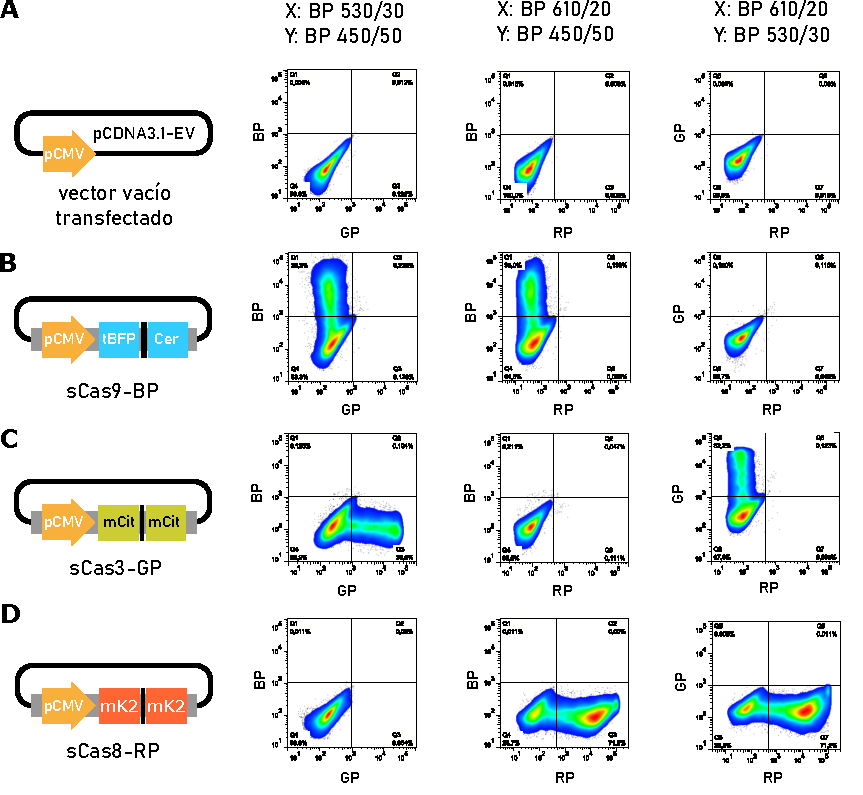
\includegraphics[width=0.9\textwidth]{img/cap_3/FACS_singles.pdf}
    \caption{\footnotesize{Se transfectaron células HeLa con un vector vacío (\textbf{A}), sCas9-BP (\textbf{B}), sCas3-GP (\textbf{C}) y sCas8-RP (\textbf{D}). En células transfectadas con un vector vacío se puede apreciar un bajo nivel de fluorescencia detectados que corresponde a autofluorescencia. En los casos de transfecciones con un único biosensor, sólo se ve un mínimo de fluorescencia correspondiente a autofluorescencia y una región intensa en el canal del biosensor transfectado, pero no en otros canales. Adaptado de \cite{Habif2021}.}}
    \label{fig:FACS_singles}
\end{figure}

\begin{figure}
    \centering
    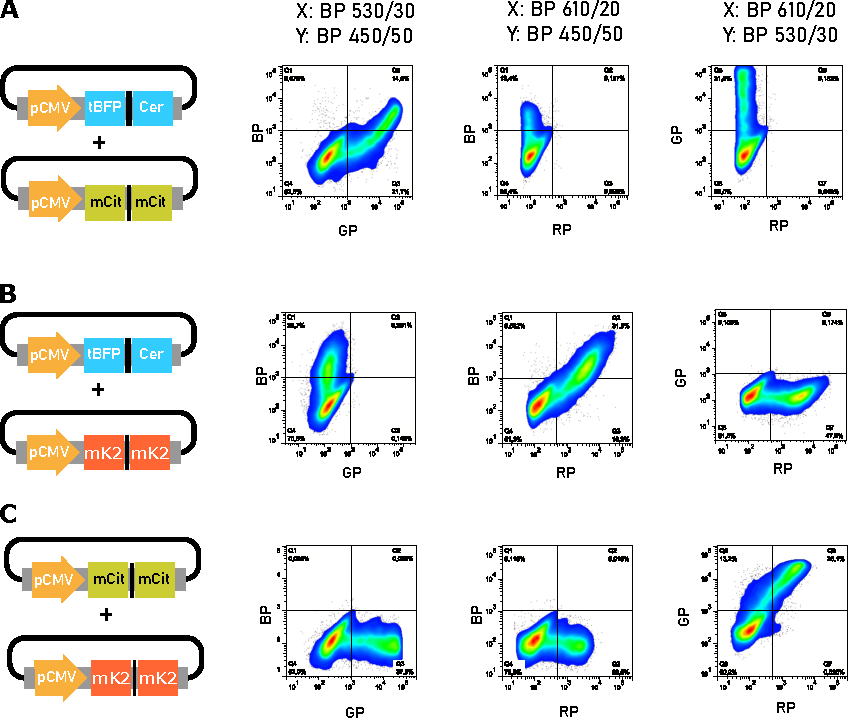
\includegraphics[width=0.9\textwidth]{img/cap_3/FACS_dobles.pdf}
    \caption{\footnotesize{Se transfectaron células HeLa con los pares de plásmidos que codifican para los biosensores: sCas3-GP + sCas9-BP (\textbf{A}), sCas3-GP + sCas8-RP (\textbf{B}) y sCas8-RP + sCas9-BP (\textbf{C}). FACS correspondiente a células transfectadas con dos biosensores en las que sólo se ve un mínimo de fluorescencia correspondiente a autofluorescencia y una región intensa que cruza entre los canales de ambos biosensores transfectados, pero no en el canal del biosensor remanente. Adaptado de \cite{Habif2021}.}}
    \label{fig:FACS_dobles}
\end{figure}

Se puede apreciar que la heterogeneidad en la expresión relativa de cada biosensor es mucho mayor en el caso de las células transfectadas con 3xCAS que con CASPAM (ver \cref{fig:FACS}). En el caso de 3xCAS, se pueden encontrar subpoblaciones que expresan sólo uno o dos sensores. Por otro lado, la relación entre las emisiones de las células transfectadas con CASPAM se conserva a lo largo de todo el rango dinámico. Aunque es sabido que la eficiencia de transfección puede mejorarse modificando el protocolo utilizado, sólo el 68,25\% las células transfectadas con 3xCAS expresaron todos los biosensores, mientras que 15,77\% expresaron sólo dos, y las restantes 15,97\% un único biosensor. En contraposición, la totalidad de las células transfectadas con CASPAM expresaron los tres biosensores (ver \cref{fig:FACS}B). Se utilizó un análisis de correlación múltiple de Pearson para cuantificar la correlación entre las intensidades detectadas obteniéndose r$_{R,GB}$=0.455, r$_{B,GR}$=0.566 y r$_{G,BR}$=0.572 para 3xCAS, mientras que para CASPAM, r$_{R,GB}$=0.962, r$_{B,GR}$=0.962 y r$_{G,BR}$=0.959, mostrando así una mejor correlación (ver \cref{fig:FACS}C). En resumen, CASPAM no solo logra coexpresar todos los biosensores, sino que también consigue un razón de coexpresión más conservada entre células.

\begin{figure}[t!]
    \centering
    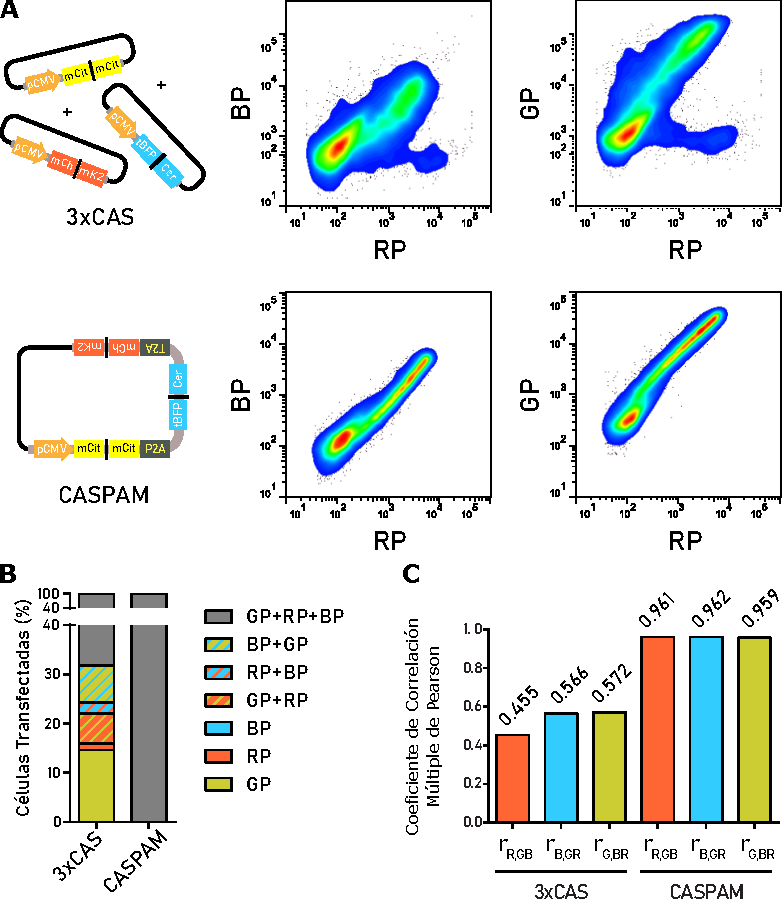
\includegraphics[width=0.8\textwidth]{img/cap_3/FACS.pdf}
    \caption{\footnotesize{Se transfectaron células HeLa con CASPAM y 3xCAS para estudiar la coexpresión a través de FACS. Adaptado de \cite{Habif2021}. \textbf{A.} En la sección superior se pueden ver los resultados del FACS en células transfectadas con 3xCAS. Además de una elevada variabilidad en la fluorescencia en la región correspondiente a células que expresan los tres biosensores, se pueden apreciar lóbulos correspondientes a células que no expresan todos los biosensores. Sin embargo, en el caso de células transfectadas con CASPAM (sección inferior), se aprecia una elevada correlación en la intensidad de fluorescencia y no se encuentran lóbulos correspondientes a células que no expresen alguno de los biosensores. \textbf{B.} Se estimó mediante ventaneo (gating) de las regiones del FACS que porcentaje de células transfectadas expresaban qué biosensores. Se vio que todas las células transfectadas con CASPAM expresaban los tres biosensores, mientras que sólo el 68,25\% las células transfectadas con 3xCAS expresaron todos los biosensores, 15,77\% expresaron sólo dos, y las restantes 15,97\% un único biosensor. \textbf{C.} Se calculó el coeficiente de correlación múltiple de Pearson para cada biosensor en ambos tipos de transfección. Se puede ver que en el caso de CASPAM, la correlación es considerablemente mayor.}}
    \label{fig:FACS}
\end{figure}


\subsection{Espectroscopia de Correlación de Fluorescencia}


\begin{figure}[b!]
    \centering
    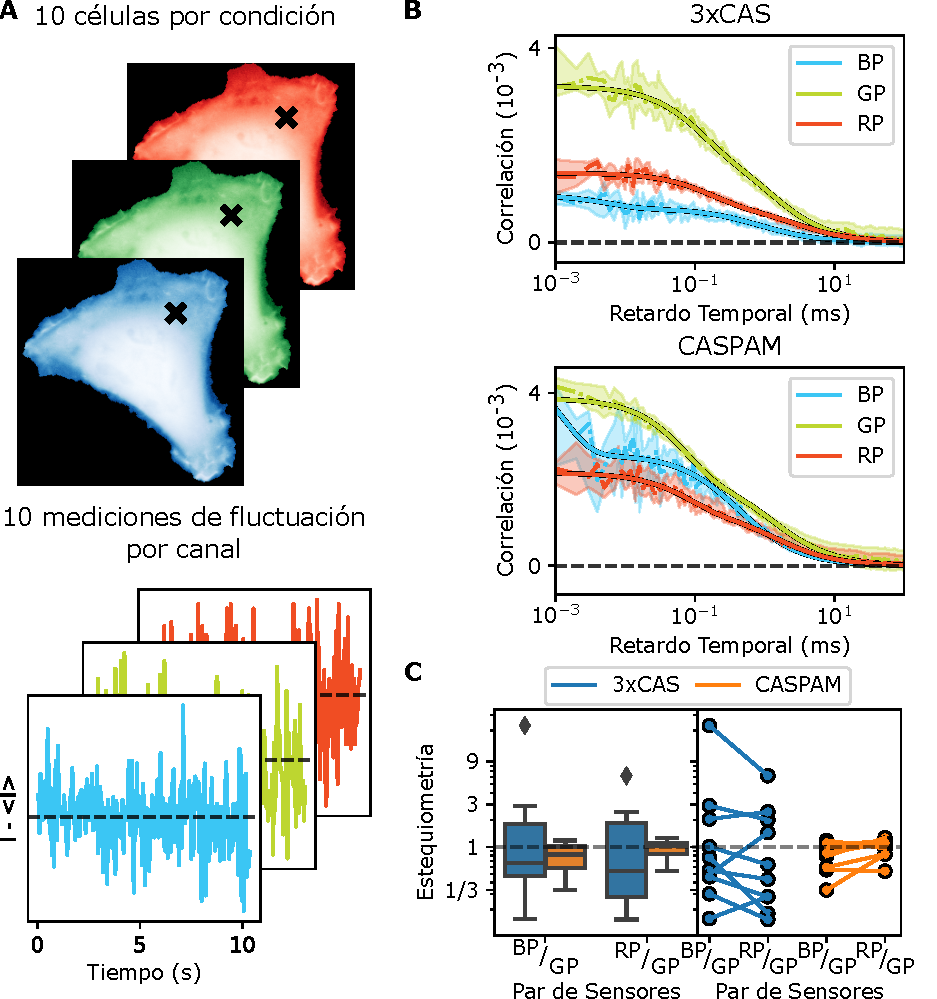
\includegraphics[width=0.8\textwidth]{img/cap_3/FCS.pdf}
    \caption{\footnotesize{Se transfectaron células HeLa con 3 CAS por separado y con CASPAM y se analizó la estequiometría de la síntesis de los biosensores. Adaptado de \cite{Habif2021}. \textbf{A.} Se analizaron 10 células de las que se adquirieron 10 repeticiones de 10 segundos de las fluctuaciones de un único punto. Como se evidencia en las figuras inferiores, no se apreció una deriva de la señal. \textbf{B.} Se calcularon las funciones de autocorrelación de cada repetición adquirida y se promediaron todas las correspondientes a un mismo punto y un mismo canal. Luego se ajustaron todas las curvas con un modelo de difusión corregido por estado triplete y se obtuvieron así los valores de G(0) y coeficientes de difusión, entre otros parámetros. \textbf{C.} Se calcularon las relaciones de concentración entre los pares de biosensores. La varianza de las relaciones de las células transfectadas con CASPAM es mucho menor que la de 3xCAS. Para  3xCAS, el intervalo intercuartil de estequiometría entre BP y GP fue de 0.47-1.79, y 0.28-1.86 para RP y GP, mientras que para CASPAM la estequiometría entre BP y GP estuvo entre 0.58-1.01 y 0.83-1.11 para RP y GP.}}
    \label{fig:FCS}
\end{figure}

En este caso se utilizó un microscopio invertido confocal de escaneo Leica TCS SP8 equipado con un láser de luz blanca pulsado de 470-670~nm (WLL2 Kit, NKT Photonics) que tenía montada una cámara de ambiente controlado (Life Imaging Services) que mantenía la temperatura a 37$^{\circ}$C. Las células se hallaban inmersas en medio DMEM (con 25~mM HEPES y sin rojo fenol). Se utilizó un objetivo HC PL APO 63x/1.4 NA CS2 de inmersión en aceite (Leica Microsystems). Las fluctuaciones de fluorescencia se obtuvieron mediante escaneo de un único punto en 10 repeticiones de 10 segundos (ver \cref{fig:FCS}A). Se calcularon las funciones de autocorrelación para cada repetición y luego se promediaron todas las funciones correspondientes a un mismo punto y canal. Para caracterizar el volumen confocal se utilizaron microesferas fluorescentes TetraSpeck de 100~nm (Invitrogen).

Se utilizó un modelo de difusión corregida por estado triplete para ajustar las funciones de autocorrelación promediadas. Dicha ecuación consiste en

\begin{equation}
    G (\tau) = G(0) \frac{(1 - F + F e^{-\tau/\tau_F})}{(1-F)} \frac{1}{(1 + (\tau / \tau_{D})) (1 + a^{-2} (\tau / \tau_{D}))^{1/2}} + G(\infty),
\end{equation}

\noindent donde $\tau$ es el retardo temporal en la autocorrelación,$\tau_D$ es el tiempo característico de difusión, $a$ es la razón $\omega_z / \omega_{xy}$ entre radio axial y lateral, $F$ es la proporción de partículas que entran en estado triplete, dejando de fluorescer, y $\tau_F$ su tiempo de relajación \citep{Widengren1995}. A partir de $G(0)$ se puede calcular la cantidad de difusores en el volumen a través de

\begin{equation}
    G(0) = \frac{1}{<N>} = \frac{1}{V_{Eff} <C>},
\end{equation}

\noindent y luego su concentración.

A partir de los ajustes, se analizaron los tiempos característicos de difusión así como la concentración de cada biosensor en cada célula. En cuanto a tiempos de difusión, aunque los volúmenes son levemente distintos entre canales, no se pudo apreciar una diferencia. Sin embargo, las concentraciones de biosensores variaban de canal a canal, así como de célula a célula. A pesar del rango dinámico considerablemente menor de FCS respecto a FACS, las células transfectadas con 3xCAS mostraron una variabilidad mucho más elevada que las transfectadas con CASPAM en la expresión relativa entre sensores (ver \cref{fig:FCS}C). En particular, para  3xCAS, la estequiometría entre BP y GP se mantuvo entre 0.47-1.79, y 0.28-1.86 para RP y GP, mientras que para CASPAM la estequiometría entre BP y GP estuvo entre 0.58-1.01 y 0.83-1.11 para RP y GP (donde los valores representan el rango intercuartil). Adicionalmente, la mediana de la expresión relativa entre cada par de biosensores de CASPAM fue cercana a la equimolaridad: 0.82 para BP y GP y 1.03 para RP y GP. Todo esto apunta a que CASPAM puede ser utilizado para obtener una co-expresión con un razón más definida entre biosensores en células individuales.


%%%%%%%%%%%%%%%%%%%%%%%%%
\section{Variabilidad en la Perturbación Introducida}


Habiendo caracterizado las mejoras introducidas por CASPAM en el control de la estequiometría, debemos corroborar dicha mejora en un experimento relevante para la biología. Para ello, se utilizaron nuevamente células transfectadas con 3xCAS o CASPAM, se las trató con staurosporina para inducir apoptosis y se las siguió mediante microscopía por 15~hr. Se analizaron las imágenes siguiendo el protocolo detallado en el capítulo \ref{cap:MatMet} y se obtuvieron los tiempos de máxima actividad de cada caspasa.

Como se discutió previamente, elevar la concentración del biosensor de alguna caspasa introducirá una demora en la propagación de la señal en la red. A modo de ejemplo, podemos tomar el modelo introducido en \cite{Corbat2018} (que será descripto en detalle en el capítulo \ref{cap:Modelos}) basado en ecuaciones diferenciales ordinarias y simular la cascada apoptótica utilizando concentraciones cada vez más altas de sCas3 (ver \cref{fig:variabilidad}A). Podemos apreciar que cambiando dicha concentración, la diferencia de tiempo entre máxima actividad de cada caspasa varía (ver \cref{fig:variabilidad}B). En la contraparte experimental, estudiaremos el impacto de seleccionar células cuya intensidad esté en un rango predefinido. Seleccionaremos células cuyo z-score de intensidad se encuentre entre -0.5 y 0.5 en cada biosensor. En efecto, debido a la elevada correlación entre la razón de intensidad de biosensores en las células transfectadas con CASPAM, seleccionar un rango de intensidad para un biosensor equivale a seleccionar un rango para los otros biosensores, a diferencia de las células transfectadas con 3xCAS. Luego de analizar el desvío estándar de las diferencias de tiempo entre los máximos de las caspasas, podemos apreciar que para CASPAM es considerablemente menor verificándose así una variabilidad menor en la perturbación introducida.

\begin{figure}[htb]
    \centering
    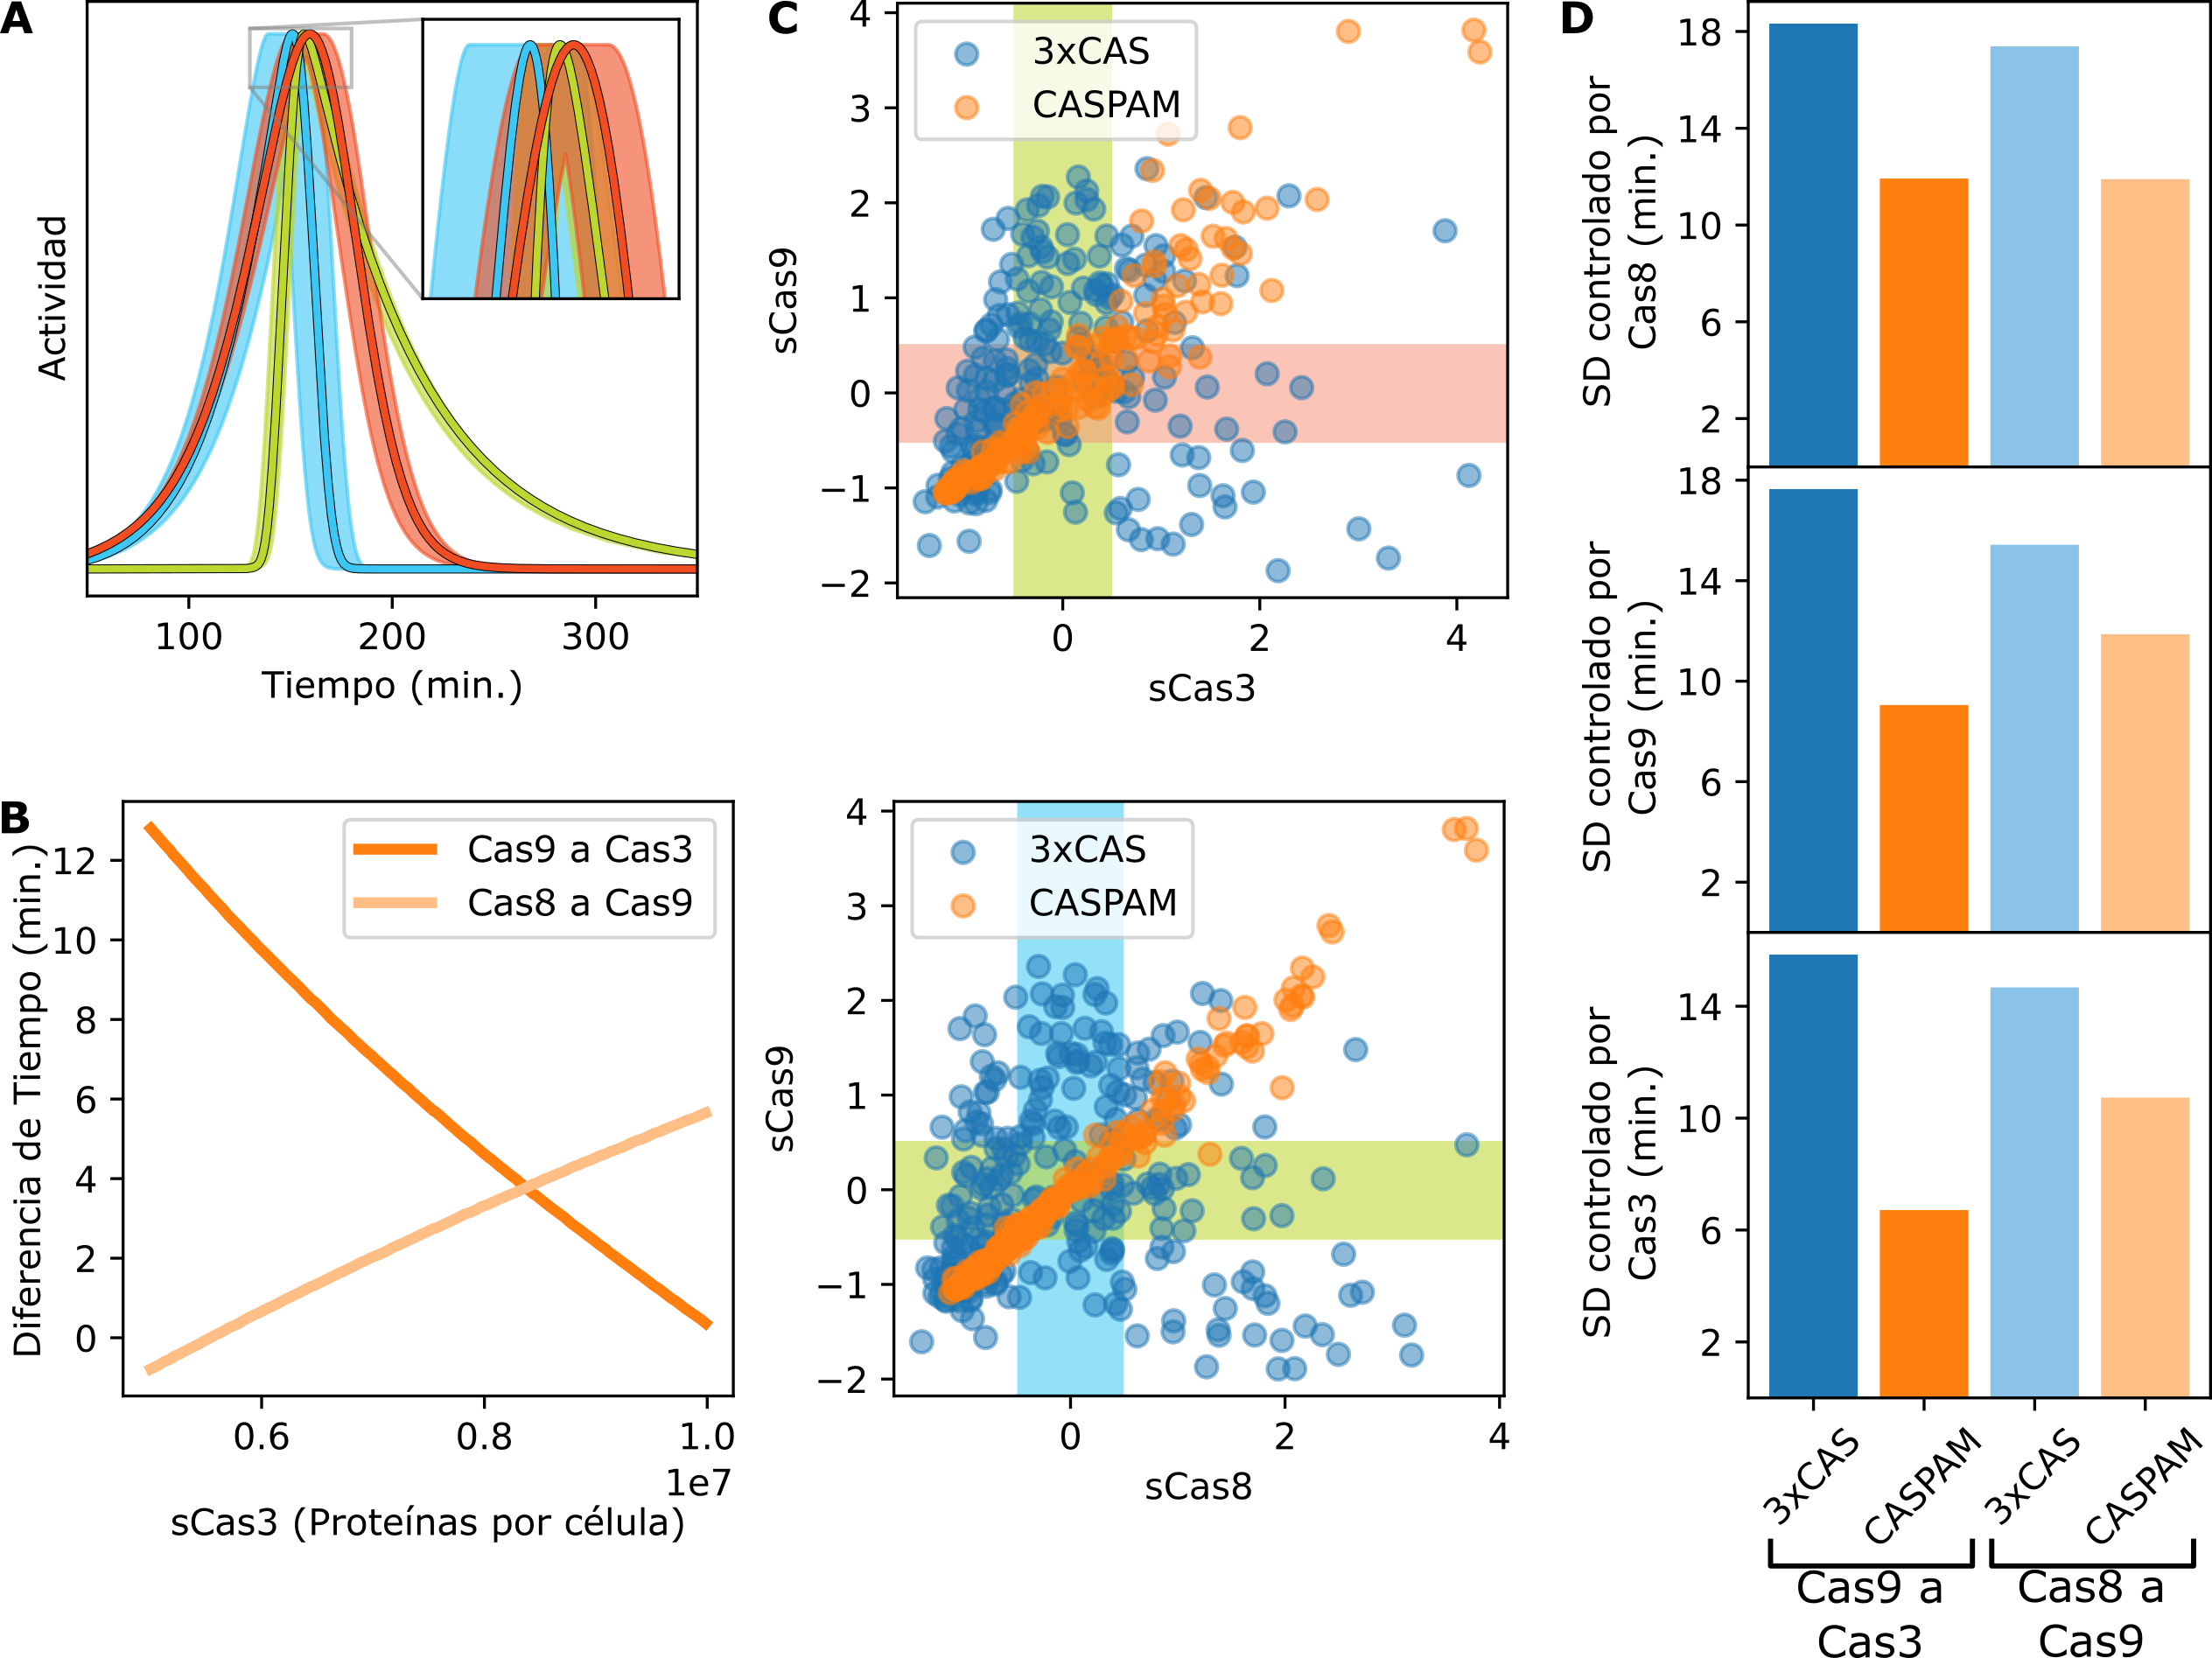
\includegraphics[width=0.9\textwidth]{img/cap_3/variabilidad.png}
    \caption{\footnotesize{Se simuló y se midió experimentalmente el efecto de introducir los biosensores con relación de estequiometría variables. Adaptado de \cite{Habif2021}. \textbf{A.} Se simularon curvas de actividad variando la concentración del biosensor sCas3 a lo largo de los valores utilizados en el modelo. La curva remarcada corresponde a la simulación con la mediana de concentración de sCas3, mientras que la región pintada engloba todas las curvas obtenidas. \textbf{B.} Se graficó la diferencia de tiempo entre los máximos de actividad de las caspasas 9 y 3 y las caspasas 8 y 9 para cada concentración de sCas3 simuladas. \textbf{C.} Se estimó la fluorescencia de cada célula transfectada con CASPAM o 3xCAS y se graficaron los z-score de cada biosensor en función de los otros. Aunque el rango dinámico de microscopía es considerablemente menor que el de FACS, todavía se aprecia una variabilidad más elevada en las células transfectadas con 3xCAS. Luego se seleccionaron 3 grupos correspondientes a los que tenían una fluorescencia cuyo z-score se hallase entre -0.5 y 0.5. \textbf{D.} Se analizó el desvió estándar de las diferencias de tiempo entre los máximos de actividad de cada caspasa y se puede ver que en todos los casos CASPAM tiene menos variabilidad en los observables que 3xCAS. Esto se debe a que al seleccionar células en cierto rango de intensidad para un biosensor de CASPAM, se seleccionan células en un rango similar en los otros biosensores, mientras que esto no sucede en 3xCAS.}}
    \label{fig:variabilidad}
\end{figure}

Dentro de todo, CASPAM permite alcanzar una expresión casi equimolar de todos los biosensores, reduciendo así la variabilidad de las perturbaciones introducidas y, por ende, los observables biológicos. Adicionalmente, conocer la concentración relativa entre los biosensores introducidos facilitará el modelado del sistema ya que reduce la cantidad de parámetros a determinar. Desde un punto de vista experimental, al utilizar CASPAM no es necesario corroborar la expresión en todos los canales ya que la totalidad de las células que expresan un biosensor, expresan los otros dos. Además, es posible seleccionar los parámetros de adquisición buscando las células más intensas en un canal y utilizándolas para verificar los parámetros en los otros canales.